\documentclass[conference]{IEEEtran}

\usepackage{graphicx}
\usepackage{amsmath,amssymb}
\usepackage{booktabs}
\usepackage{array}
\usepackage{cite}
\usepackage{url}
\usepackage{balance}
\usepackage{microtype}
\usepackage{listings}
\usepackage{tikz}
\usetikzlibrary{arrows.meta,positioning}


\title{Dataset-Specialised TabICL: Dataset Representation Learning, Expert Specialisation, and Retrieval-Based Prediction}

\author{
\IEEEauthorblockN{
Ayinala Sri Nikesh (240041005)\\
Geddada Mahidhar (240041017)\\
Kesavarapu Deepak Reddy (240041022)
}
\IEEEauthorblockA{
MA 305 -- Data Science Project\\
End Evaluation -- Team 7\\
\url{https://github.com/Mahidhar21/Dataset-Specialised-TabICL}
}
}

\begin{document}
\maketitle

\begin{abstract}
We investigate dataset-specialised TabICL through fixed-dimensional dataset representations, cluster-based expert training, and retrieval-based prediction. On 67 numerical-only binary-classification datasets, we compare 88-dimensional statistical meta-features with 512-dimensional mean-pooled and 1024-dimensional mean--standard-deviation pretrained TabICL representations. Mean pooling achieves within-dataset cosine similarity of 0.938 and 33/36 nearest-neighbour identifications under context resampling. A family-aware split assigns 53 meta-training datasets to four K-means clusters (16, 15, 12, 10), leaving 14 datasets for testing. Four TabICL v2 expert checkpoints are produced by independent episodic fine-tuning with validation-based selection, including the pretrained initialization as a candidate. Nearest-centroid top-three aggregation achieves mean accuracy of 86.33\%, compared with 86.16\% for pretrained TabICL, 86.22\% for random top-three and 86.38\% for fixed top-three. The pretrained model retains better balanced accuracy, macro-F1, and log loss. Separately, a 32-estimator TabICL v1 benchmark completes 188 of 200 TALENT tasks, obtaining 83.48\% mean accuracy, 0.8936 macro AUC, 0.3796 log loss and 12.57 s median runtime. The two protocols are not directly comparable. These results establish end-to-end feasibility but do not establish a reliable predictive or routing advantage.
\end{abstract}

\begin{IEEEkeywords}
TabICL, tabular in-context learning, dataset embeddings, meta-features, dataset clustering, expert routing, TALENT benchmarking
\end{IEEEkeywords}

\section{Introduction}

Tabular in-context learning with TabICL~\cite{tabicl} provides a foundation for this work. Tabular classification tasks differ in sample count, dimensionality, feature distributions, and target structure. A general pretrained tabular in-context learning model offers a convenient starting point, yet its behaviour may vary across such tasks.

Our project investigates whether a dataset can first be represented as an object in a shared embedding space and then routed to a specialised version of TabICL.

The ultimate objective is not simply to discover clusters, but to determine whether expert specialisation improves predictive performance on previously unseen datasets.

The proposed system has four stages:

\begin{enumerate}
\item Dataset Representation Learning.
\item Dataset Clustering and Expert Assignment.
\item Joint Multi-Dataset Expert Training.
\item Retrieval-Based Expert Selection and Prediction.
\end{enumerate}

This report documents all four implemented stages and distinguishes exploratory embedding and clustering metrics from held-out predictive evaluation.

Our contributions are fivefold. First, we construct and align multiple fixed-dimensional representations of 67 binary-classification datasets. Second, we quantify the sensitivity of pooled TabICL embeddings to context-row resampling. Third, we implement family-aware partitioning and training-only clustering. Fourth, we implement independent multi-dataset fine-tuning, nearest-centroid prediction, and random and fixed routing controls. Fifth, a separate team benchmark characterises pretrained TabICL v1 on 188 completed TALENT tasks.

The consolidated source code and recorded experimental artifacts are maintained in the project repository~\cite{project}:

\url{https://github.com/Mahidhar21/Dataset-Specialised-TabICL}

\section{Problem Formulation and Architecture}

Let the meta-training collection be

\begin{equation}
\mathcal{D} = \{D_1,D_2,\ldots,D_M\},
\end{equation}

where each dataset is

\begin{equation}
D_i=(X_i,y_i),
\quad X_i\in\mathbb{R}^{n_i\times d_i}.
\end{equation}

A dataset encoder $g$ produces a fixed-dimensional embedding

\begin{equation}
z_i=g(D_i)\in\mathbb{R}^{p}.
\end{equation}

Clustering assigns each meta-training dataset to one of $K$ groups

\begin{equation}
C_1,C_2,\ldots,C_K.
\end{equation}

Each cluster corresponds to a specialised TabICL expert $E_j$.

The central downstream question is whether a routing function $r(D_q)$ can select an expert that performs better on an unseen query dataset $D_q$ than the unmodified pretrained TabICL model.

\subsection{Four-Stage Architecture}
The implementation uses the pretrained TabICL v2 row-interactor as a fixed representation extractor, followed by standardisation and ordinary K-means. Each cluster defines an independent expert initialized from the same pretrained checkpoint. At inference, the same representation extractor and fitted router rank the experts; selected models predict using labelled support rows, and their probabilities are averaged.
\begin{figure}[t]
\centering
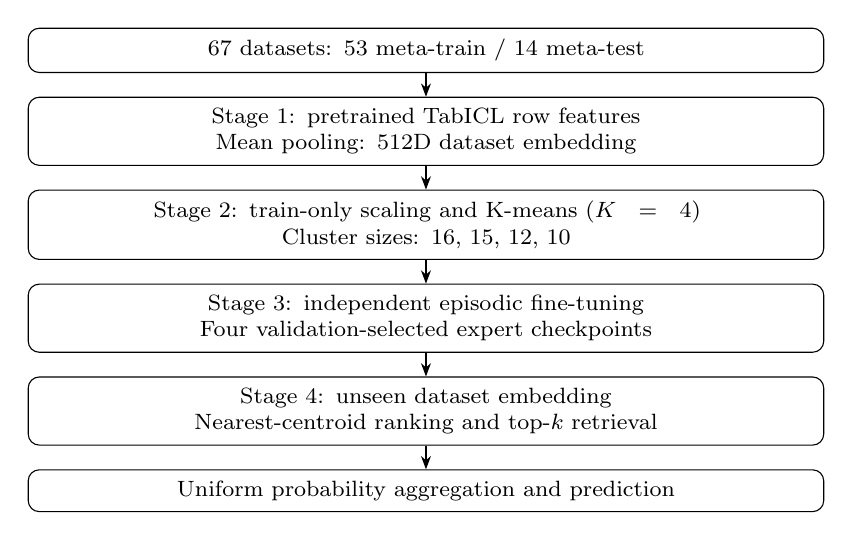
\begin{tikzpicture}[node distance=3mm, every node/.style={font=\footnotesize}, block/.style={draw, rounded corners, align=center,text width=0.81\columnwidth,inner sep=4pt}, >={Stealth}]
\node[block] (a) {67 datasets: 53 meta-train / 14 meta-test};
\node[block,below=of a] (b) {Stage 1: pretrained TabICL row features\\Mean pooling: 512D dataset embedding};
\node[block,below=of b] (c) {Stage 2: train-only scaling and K-means ($K=4$)\\Cluster sizes: 16, 15, 12, 10};
\node[block,below=of c] (d) {Stage 3: independent episodic fine-tuning\\Four validation-selected expert checkpoints};
\node[block,below=of d] (e) {Stage 4: unseen dataset embedding\\Nearest-centroid ranking and top-$k$ retrieval};
\node[block,below=of e] (f) {Uniform probability aggregation and prediction};
\foreach \u/\v in {a/b,b/c,c/d,d/e,e/f}{\draw[->] (\u)--(\v);}
\end{tikzpicture}
\caption{Implemented architecture. Meta-test datasets do not contribute to centroid fitting or expert weight updates. At inference, the fitted representation and router are reused.}
\label{fig:architecture}
\end{figure}
The original design proposes approximately balanced clustering and learned gating as possible extensions. Neither is evaluated here.

\section{Dataset Representation Learning}

\subsection{Dataset Collection}

The initial benchmark consists of 67 numerical-only binary-classification datasets.

Each dataset has its own feature dimension and number of observations. Consequently, directly concatenating rows across datasets cannot define a uniform dataset representation.

Instead, we compute fixed-dimensional per-dataset summaries.

Name-index alignment is enforced when comparing statistical and TabICL representation matrices.

The pilot uses available dataset training arrays for embedding extraction. The downstream implementation uses 256 stratified context rows and one additional unlabelled row to trigger the forward hook. The additional row is excluded from mean pooling.

\subsection{Statistical Meta-Features}

The first representation strategy uses statistical characteristics of each dataset.

A statistical encoder maps dataset $D_i$ into

\begin{equation}
z_i^{stat}\in\mathbb{R}^{88}.
\end{equation}

This provides a non-neural baseline based on tabular characteristics.

Different scaling choices are important because dataset statistics can vary by orders of magnitude.

Our exploratory comparison includes standard scaling, signed-log transformation, and robust scaling.

For a scalar $x$, the signed-log transformation is

\begin{equation}
T(x)=\operatorname{sign}(x)\log(1+|x|).
\end{equation}

Although some statistical features were imputed during earlier global extraction, a strictly held-out final analysis must refit cross-dataset imputation using meta-training datasets alone.

\subsection{TabICL-Based Dataset Embeddings}

The second representation strategy extracts intermediate features from the pretrained TabICL model.

A forward hook on the row-interaction module produces row representations

\begin{equation}
h_{ir}\in\mathbb{R}^{512}.
\end{equation}

For $m$ sampled context rows, mean pooling produces

\begin{equation}
z_i^{mean}
=
\frac{1}{m}
\sum_{r=1}^{m}h_{ir}.
\end{equation}

The resulting representation is

\begin{equation}
z_i^{mean}\in\mathbb{R}^{512}.
\end{equation}

An alternative representation concatenates the coordinate-wise mean and standard deviation:

\begin{equation}
z_i^{mean+std}
=
[\mu_i;\sigma_i]
\in\mathbb{R}^{1024}.
\end{equation}

Both approaches generate fixed-dimensional representations independent of the original dataset size. We regenerate all 67 mean embeddings on CPU, using seed 42 and one TabICL estimator, and reproduce all 53 committed training cluster assignments (zero mismatches).

Pooling is permutation-invariant over the extracted row features, although the upstream TabICL computation may still depend on preprocessing, sampling, and randomness.

These intermediate representations should not automatically be interpreted as explicitly target-aware dataset embeddings.

\subsection{Embedding Stability Experiment}

To evaluate embedding consistency, we performed a row-resampling experiment.

Twelve datasets were selected, with three independent context samples per dataset. Each sample used 128 context rows and varying random seeds.

This produced 36 embeddings for each representation strategy.

We measured within-dataset cosine similarity, between-dataset cosine similarity, and nearest-neighbour identification accuracy.

\begin{table}[t]
\caption{Row-Resampling Stability Results}
\label{tab:stability}
\centering
\footnotesize
\begin{tabular}{lrrrr}
\toprule
Representation & Within & Between & Gap & NN Match\\
\midrule
Mean (512D) & .938 & .747 & .191 & 33/36\\
Mean+std (1024D) & .945 & .792 & .153 & 32/36\\
\bottomrule
\end{tabular}
\end{table}

Mean+std pooling produces slightly higher within-dataset similarity. However, mean pooling produces a larger within-versus-between similarity gap and better nearest-neighbour identification accuracy.

The mean representation achieves 91.67\% nearest-neighbour accuracy, compared with 88.89\% for mean+std.

Therefore, we select 512-dimensional mean pooling as the primary representation, retaining mean+std as an ablation.

These results measure representation stability rather than downstream predictive performance.

\begin{figure}[t]
\centering
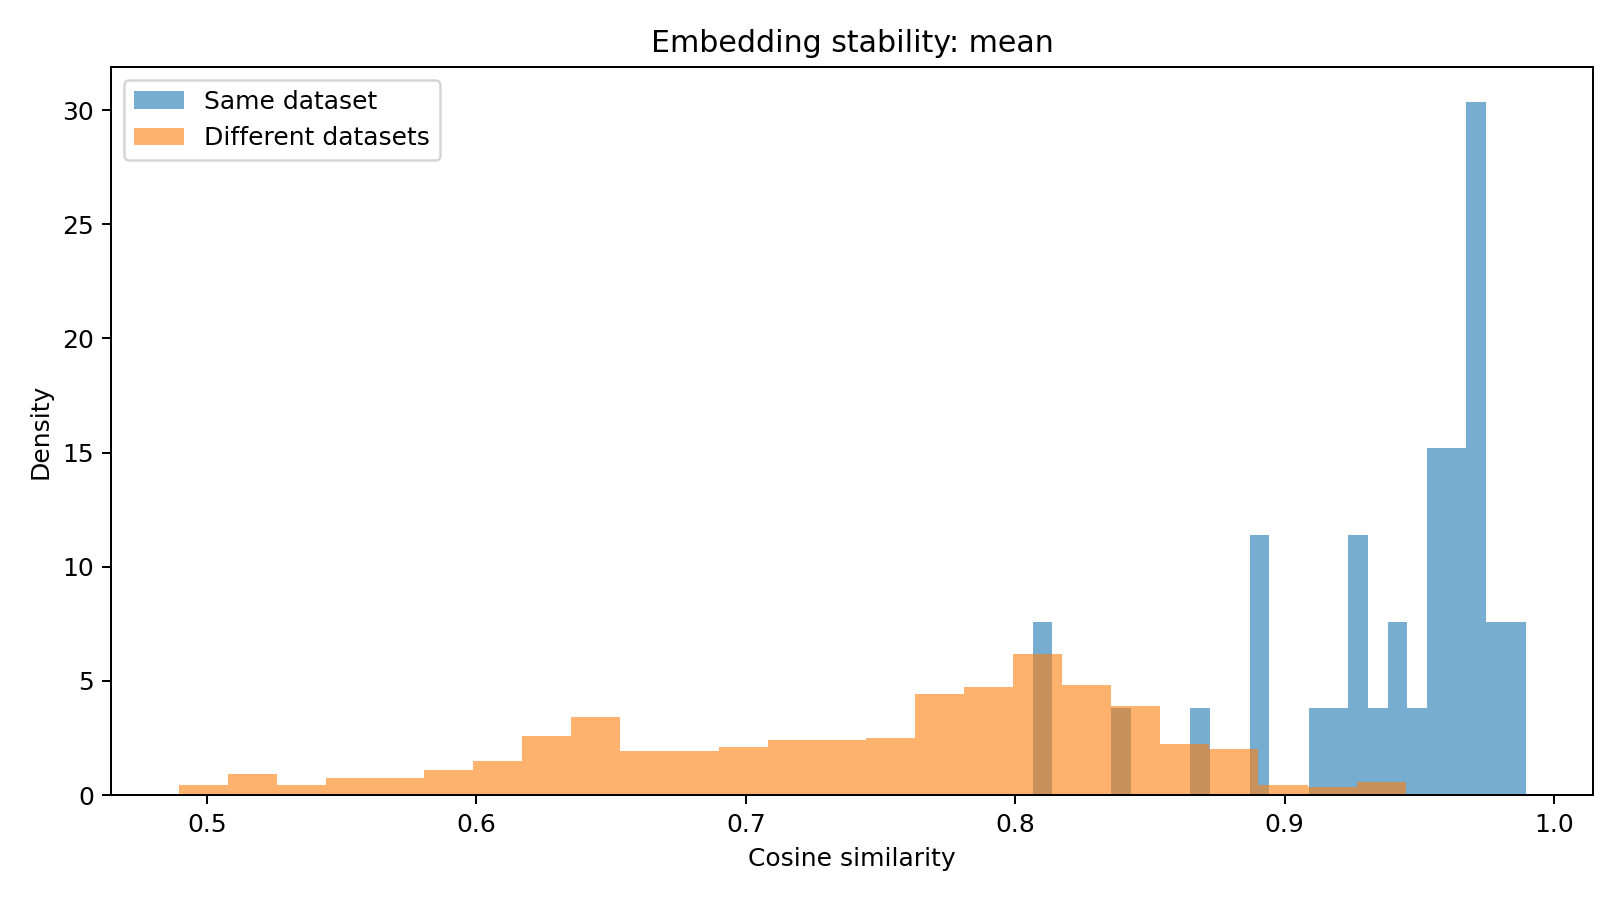
\includegraphics[width=\columnwidth]{figures/similarity_mean.png}
\caption{Cosine similarity structure for 512D mean-pooled TabICL embeddings across resampled dataset contexts.}
\label{fig:similarity_mean}
\end{figure}

\section{Dataset Clustering and Expert Assignment}

\subsection{K-Means Clustering}

After extracting dataset embeddings, we apply K-means clustering to group datasets with similar representations.

After removing near-constant embedding coordinates (training variance at most $10^{-12}$), the final implementation fits a StandardScaler on meta-training embeddings. Writing $\widetilde z_i$ for the transformed vector, the objective of K-means is

\begin{equation}
\min_{\{\mu_j\},\{a_{ij}\}}
\sum_{i=1}^{M}
\sum_{j=1}^{K}
a_{ij}
\left\|\widetilde z_i-\mu_j\right\|_2^2,
\end{equation}

where $\mu_j$ represents cluster centroid $j$ and $a_{ij}$ indicates whether dataset $i$ belongs to cluster $j$, with $a_{ij}\in\{0,1\}$ and $\sum_j a_{ij}=1$. The final K-means fit uses seed 42 and 20 initializations.

We initially explored $K=8$ with multiple representations and normalisation methods.

Clustering was evaluated using silhouette score, adjusted Rand index (ARI), cluster-size distribution, nearest-neighbour relationships, and PCA visualisations.

\subsection{Exploratory Results for K=8}

Table~\ref{tab:k8} presents selected exploratory clustering results.

\begin{table}[t]
\caption{Selected Exploratory Results for K=8}
\label{tab:k8}
\centering
\footnotesize
\begin{tabular}{lrrr}
\toprule
Configuration & Silhouette & ARI & Size Range\\
\midrule
Statistical robust & .829 & 1.000 & 1--57\\
Statistical signed-log & .205 & .648 & 1--15\\
TabICL mean, unit norm & .133 & .659 & 1--14\\
TabICL mean, standard & .106 & .538 & 2--17\\
TabICL mean+std, standard & .076 & .495 & 4--13\\
\bottomrule
\end{tabular}
\end{table}

Although robust-scaled statistical features achieved a high silhouette score of 0.829, the resulting clustering was highly imbalanced.

One cluster contained 57 datasets, while six clusters contained only one dataset each.

This illustrates why silhouette score alone is insufficient for determining useful expert groups.

Several K=8 configurations produced small clusters, which could make specialised expert training difficult.

\begin{figure}[t]
\centering
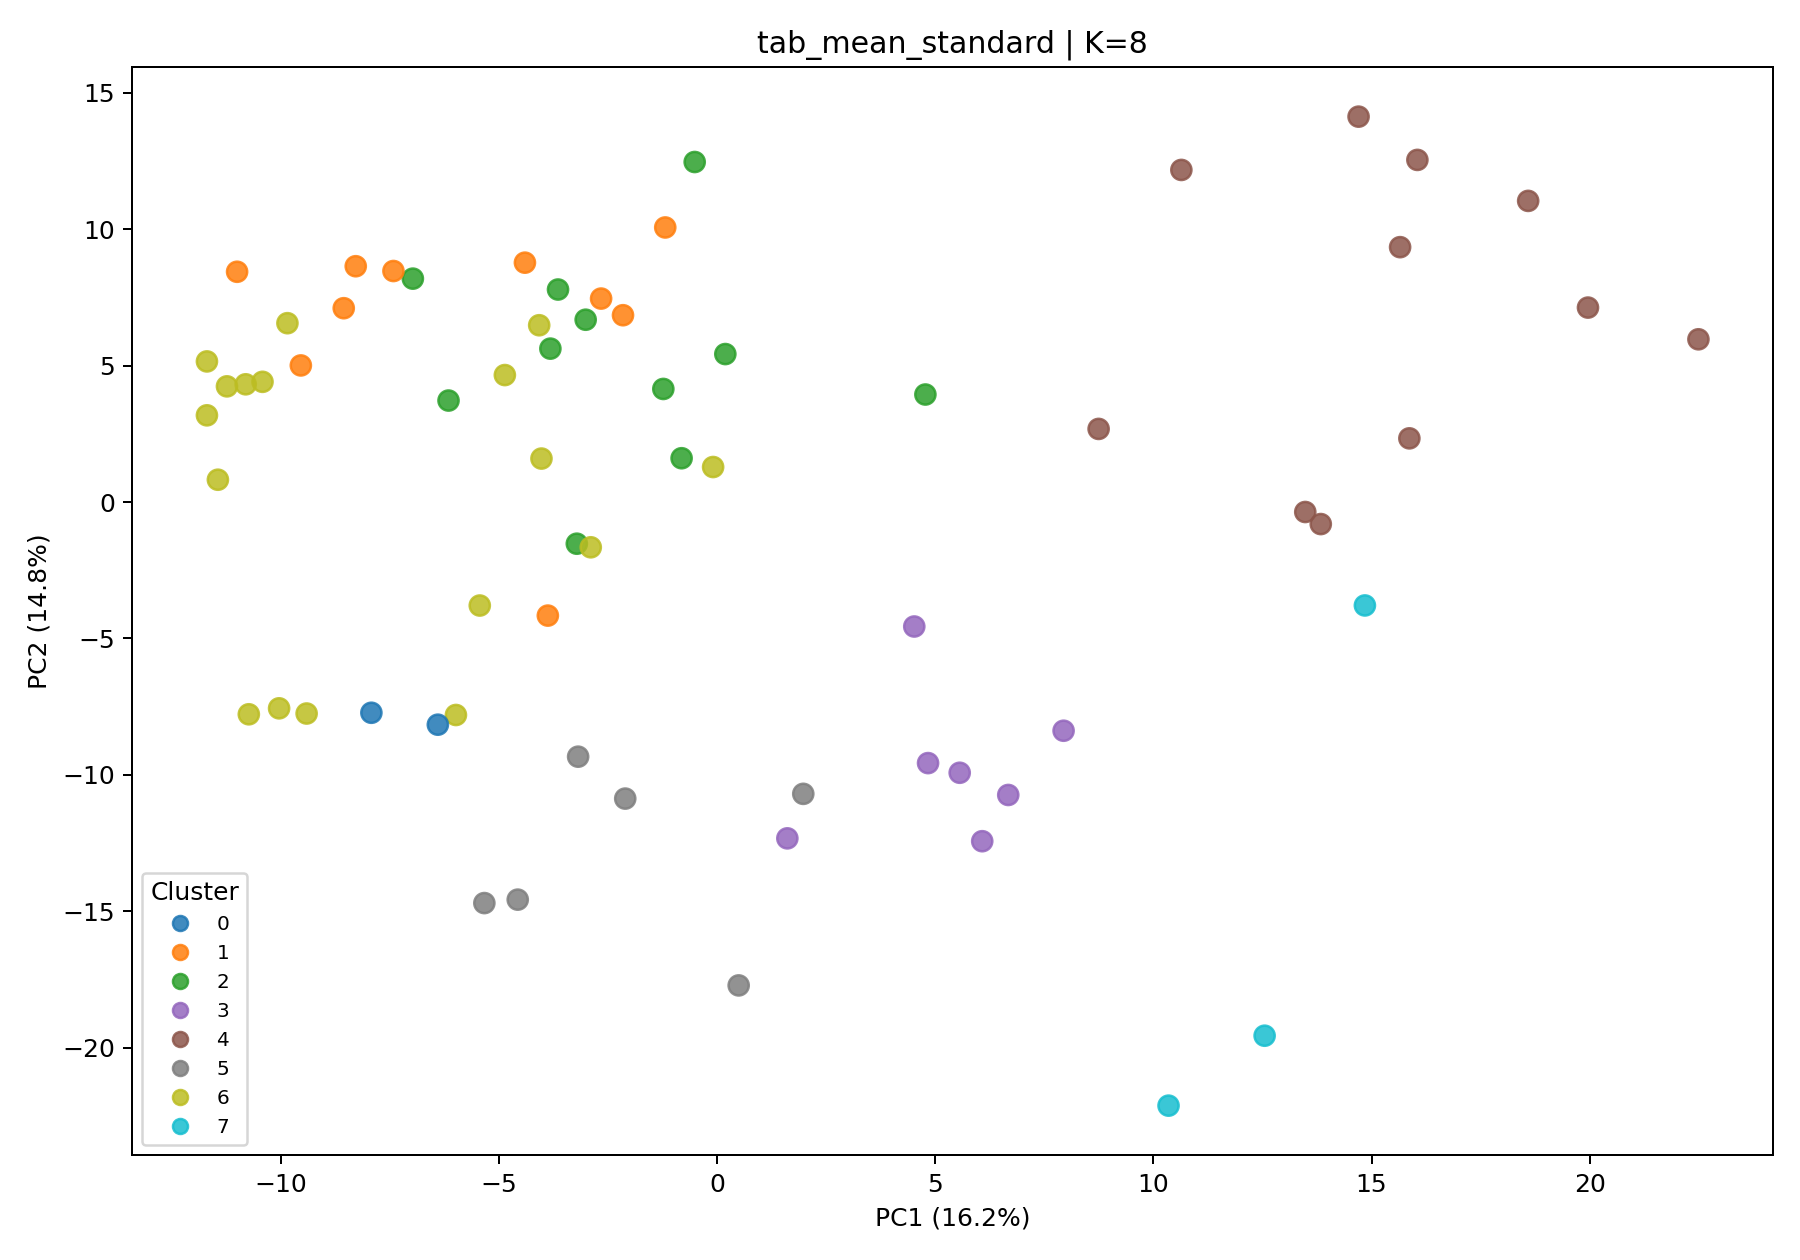
\includegraphics[width=\columnwidth]{figures/pca_tab_mean_standard.png}
\caption{Exploratory PCA projection of standardised 512D TabICL mean embeddings for K=8 clustering.}
\label{fig:pca_mean}
\end{figure}

\subsection{Family-Aware Dataset Splitting}

Closely related dataset variants may introduce evaluation leakage if they appear in both meta-training and meta-test partitions.

To reduce this risk, we implemented group-aware dataset splitting.

Known related groups include FOREX variants, microwave-sensing datasets at different frequencies, the \texttt{ada} variants, and a conservatively grouped set of software-defect datasets.

These family definitions are heuristic and should be reviewed against dataset provenance before final publication.

The revised K=4 experiment contains:

\begin{itemize}
\item 53 meta-training datasets.
\item 14 held-out meta-test datasets.
\end{itemize}

Preprocessing and K-means centroids are fitted using meta-training datasets only.

Held-out dataset embeddings are assigned to the nearest fitted centroid without updating the clustering model.

Five held-out datasets belong to the microwave-sensing family, motivating family-level aggregation in future evaluation.

\subsection{Final Prototype Configuration: K=4}

To avoid extremely small expert groups, we selected K=4 as the primary prototype configuration.

The resulting cluster sizes are shown in Table~\ref{tab:k4}.

\begin{table}[t]
\caption{Meta-Training Cluster Sizes for K=4}
\label{tab:k4}
\centering
\footnotesize
\begin{tabular}{lrrrr}
\toprule
Representation & $C_0$ & $C_1$ & $C_2$ & $C_3$\\
\midrule
Statistical signed-log & 22 & 11 & 14 & 6\\
TabICL mean & 16 & 15 & 12 & 10\\
TabICL mean+std & 21 & 16 & 9 & 7\\
\bottomrule
\end{tabular}
\end{table}

The 512D mean-pooled TabICL representation produces four clusters containing 16, 15, 12, and 10 datasets.

Unlike K=8, this configuration avoids singleton clusters.

Therefore, the working configuration for subsequent experiments is:

\begin{equation}
\boxed{
\text{TabICL Mean Embeddings}
+
\text{K-Means}(K=4)
}
\end{equation}

However, K=4 and K=8 were evaluated using different family-aware splits.

Consequently, these results support a practical training-feasibility decision but do not establish that K=4 is statistically or predictively superior to K=8.

\section{Joint Multi-Dataset Expert Training}
Each expert $E_j$ ($j=0,1,2,3$) starts from the same pretrained TabICL v2 classifier checkpoint, \texttt{tabicl-classifier-v2-20260212.ckpt}. Within each cluster, a family-aware validation split is made before weight updates. The resulting training/validation dataset counts are $(13,3)$, $(11,4)$, $(9,3)$, and $(9,1)$. No meta-test dataset contributes to weight updates or checkpoint selection. The column embedder and row interactor are frozen; the ICL predictor is trainable (26,276,362 parameters per expert).

\subsection{Training Objective and Loop}
Rather than concatenating heterogeneous tables, each step samples one training dataset uniformly from the assigned cluster. A stratified 64-row subset is sampled, and at most 32 features are randomly selected. The upstream meta-batch generator constructs a context/query episode with query ratio 0.25 (nominally 48 context and 16 query rows), one estimator, and feature/class permutations. The expert predicts query labels conditioned on labelled context. For classification, the objective is
\begin{equation}
\begin{aligned}
\mathcal L_j(\theta_j)&=\mathbb E_{D_i\sim P_j,\,T\sim D_i}[\ell_j(T)],\\
\ell_j(T)&=-\frac{1}{|Q|}\sum_{r\in Q}\log p_{\theta_j}(y_r\mid X_C,y_C,x_r).
\end{aligned}
\end{equation}
Here $C,Q$ are the context and query index sets after episode construction. Parameters are updated independently using AdamW, learning rate $10^{-5}$, weight decay 0.01, gradient clipping at norm 1, and CUDA FP16 automatic mixed precision with gradient scaling.

\begin{table}[t]
\caption{Expert Training Configuration}
\centering\footnotesize
\begin{tabular}{ll}\toprule
Setting & Value\\\midrule
Hardware & RTX 3050 Laptop GPU (6 GB)\\
Epochs / steps per epoch & 3 / 30\\
Episode rows / feature cap & 64 / 32\\
Query fraction & 0.25\\
Learning rate / weight decay & $10^{-5}$ / 0.01\\
Trainable parameters & 26,276,362\\
Validation split target & 20\% of families\\
Base seed & 42\\\bottomrule
\end{tabular}
\end{table}

The implementation uses the native TabICL fine-tuning helpers in a custom multi-dataset loop. Each step resamples invalid episodes (up to 20 attempts), clears gradients, backpropagates the scaled loss, unscales and clips gradients, then applies the optimizer update. Validation uses a fixed episode seed per validation dataset, without gradients. The initialization is evaluated before training so a checkpoint is retained only when validation loss improves. The following pseudocode summarises the actual loop (omitting retry handling and mixed-precision details).
\begin{lstlisting}[basicstyle=\ttfamily\scriptsize,breaklines=true,frame=single]
for j in range(4):
    model = load_pretrained()
    freeze_column_and_row(model)
    train, val = family_split(cluster[j])
    best = validate(model, val)
    save_best(model)
    for epoch in range(3):
        for step in range(30):
            D = sample_uniform(train)
            batch = make_meta_batch(D)
            loss = cross_entropy(model, batch)
            optimizer.zero_grad()
            loss.backward()
            clip_grad_norm(1.0)
            optimizer.step()
        v = validate(model, val)
        if v < best:
            best = v
            save_best(model)
\end{lstlisting}
All four runs reported 90 completed training steps with zero skipped steps (360 total). The best validation checkpoints are shown in Table~\ref{tab:expertval}. Expert 2 retained the pretrained initialization; thus four expert slots were produced, but only three selected checkpoints contain fine-tuned weights.
\begin{table}[t]
\caption{Validation Loss and Checkpoint Selection}
\label{tab:expertval}
\centering\footnotesize
\begin{tabular}{lrrrrr}\toprule
Expert & Train/val & Initial & Ep. 1 & Ep. 2 & Ep. 3\\\midrule
0 & 13/3 & .3707 & .3322 & .3298 & \textbf{.3266}\\
1 & 11/4 & .3587 & .3092 & \textbf{.2921} & .3030\\
2 & 9/3 & \textbf{.1772} & .2013 & .1846 & .1884\\
3 & 9/1 & .7525 & .7283 & \textbf{.6568} & .6740\\\bottomrule
\end{tabular}
\end{table}

\section{Retrieval-Based Expert Selection and Prediction}
For a meta-test dataset, the evaluator draws 256 stratified labelled support rows using seed 42 and selects the first 128 remaining rows as queries. Pretrained TabICL yields a mean-pooled 512D embedding, using one additional unlabelled row to invoke the row-interactor hook. The saved training-fitted feature mask and scaler transform this vector into $\widetilde z_q$. Expert ranking uses Euclidean distance in the standardised space (not cosine similarity):
\begin{equation}
r(D_q)=\arg\min_{j\in\{0,1,2,3\}}\|\widetilde z_q-\mu_j\|_2^2.
\end{equation}
The top-$k$ experts are the $k$ smallest distances. Each expert receives the identical support and query features. Class probabilities are aligned to a common class order and combined uniformly:
\begin{equation}
\begin{aligned}
\bar p(y\mid x,D_q)&=\frac1k\sum_{j\in\mathcal R_k(D_q)}p_j(y\mid x,D_q),\\
\widehat y&=\arg\max_y\bar p(y\mid x,D_q).
\end{aligned}
\end{equation}
All predictive models use one estimator, batch size one, and CUDA mixed precision; weights are loaded sequentially. The original pretrained checkpoint is evaluated using exactly the same episode. Random top-three (seed 42) and a diagnostic fixed set $\{0,1,2\}$ provide routing controls. The fixed set was chosen after inspecting the initial routing selections, so it is not an independently preregistered control. The procedure does not use query labels to rank experts or compute predictions, although full dataset labels are used for stratified splitting.

\section{Downstream Experimental Evaluation}
All 14 meta-test datasets completed evaluation. Reported metrics are arithmetic means of per-dataset accuracy, balanced accuracy, macro-F1, and log loss. Higher is better for the first three; lower is better for log loss. The protocol uses held-out rows of the original training arrays, not the official benchmark test partitions.
\begin{table*}[t]
\caption{Held-Out Predictive Results (14 Datasets; Accuracy, Balanced Accuracy and Macro-F1 in Percent)}
\label{tab:results}
\centering\small
\begin{tabular}{lrrrr}\toprule
Method & Accuracy & Balanced accuracy & Macro-F1 & Log loss\\\midrule
Original pretrained TabICL v2 & 86.16 & \textbf{82.39} & \textbf{82.02} & \textbf{0.28946}\\
Nearest top-1 & 85.71 & 80.79 & 80.76 & 0.29900\\
Nearest top-3 & 86.33 & 81.76 & 81.44 & 0.29054\\
Random top-1 & 86.22 & 82.15 & 81.54 & 0.29314\\
Random top-3 & 86.22 & 81.12 & 80.92 & 0.29056\\
Fixed top-1 (expert 0) & 86.22 & 81.15 & 81.04 & 0.29795\\
Fixed top-3 (experts 0,1,2) & \textbf{86.38} & 81.88 & 81.64 & 0.29105\\\bottomrule
\end{tabular}
\end{table*}
Nearest top-three gains 0.167 percentage points in accuracy over pretrained TabICL, but loses 0.622 points in balanced accuracy and 0.582 points in macro-F1, with log loss increasing by 0.00108. Fixed top-three slightly exceeds nearest top-three in accuracy and macro-F1, while nearest top-three has marginally lower log loss among the three top-three ensembles. No significance test has been conducted; the measured differences do not establish a reliable advantage. With four experts and $k=3$, the control ensembles overlap substantially, limiting the discrimination of this routing experiment.

\section{Independent TALENT Benchmarking of TabICL v1}
\label{sec:talent}
A complementary team experiment characterises the original TabICL v1 classifier on the TALENT benchmark, independently of the v2 expert-specialisation pipeline. The analysis uses saved results in the supplied benchmarking report~\cite{talentreport} and workbook~\cite{talentworkbook}; no model inference was rerun for this synthesis. The purpose is to measure generalist predictive behaviour and practical runtime across a broad inventory of binary and multiclass tasks, not to establish the benefit of the proposed routing system.

\subsection{Protocol and Coverage}
The benchmark attempts 200 classification tasks using the official training and test partitions, with validation unused. Numerical features are cast to floating point and categorical features to strings while preserving missing values. Unlike the specialist experiment, all available training and test rows are used, and no task-specific gradient fine-tuning is performed. Table~\ref{tab:talentconfig} records the configuration reported by the benchmarking teammate.
\begin{table}[t]
\caption{Independent TALENT Benchmark Configuration}
\label{tab:talentconfig}
\centering\footnotesize
\begin{tabular}{@{}lp{0.56\columnwidth}@{}}\toprule
Setting & Value\\\midrule
Model & TabICL v1 (2025-02-08 checkpoint)\\
Estimators / seed & 32 / 42\\
Batch size / AMP & 1 / disabled\\
Hardware & NVIDIA Tesla T4 (CUDA)\\
PyTorch / sklearn & 2.14.1+cu130 / 1.6.1\\
Partitions & Official train and test; no validation tuning\\
Timing & Fit and probability prediction only\\\bottomrule
\end{tabular}
\end{table}

The supplied workbook records 187 scored and 13 pending tasks. The benchmarking report reconciles this snapshot against 188 completed JSON records, identifying \texttt{philippine} as the additional binary task (75.15\% accuracy, AUC 0.8356, log loss 0.4955, runtime 107.54 s, rounded). We independently checked the workbook counts and recomputed its scored-row aggregates: 83.52\% accuracy, 0.8939 AUC, 0.3790 log loss, and 12.54 s median runtime. The headline results below use the later 188-record report, not a mixture of denominators. The benchmarking notebook is included in the consolidated repository and was reviewed statically. The original 188 JSON records are unavailable for this synthesis, so the full-precision values and reconciliation cannot be independently audited here. The remaining 12 tasks are excluded from all headline aggregates, rather than counted as zero. Completion coverage is 94\%.

\subsection{Metrics and Results}
For task $d$ with $n_d$ test rows and class probabilities $p_{ic}$, accuracy and log loss are
\begin{equation}
 A_d=\frac{1}{n_d}\sum_i\mathbf 1[\arg\max_c p_{ic}=y_i],\quad
 L_d=-\frac{1}{n_d}\sum_i\log p_{i,y_i}.
\end{equation}
Macro one-vs-rest AUC averages the binary ranking AUC across classes with both positives and negatives in the test set; the report states that all recorded classes were included for every completed task. Each task receives equal weight in the predictive metric means, and runtime is summarised separately. These means are not pooled AUCs.
\begin{table}[t]
\caption{TALENT v1: Completed-Task Results (188/200)}
\label{tab:talentresults}
\centering\footnotesize
\setlength{\tabcolsep}{3pt}
\begin{tabular}{lrrrrr}\toprule
Subset & $N$ & Acc.(\%) & AUC & Loss & Med. s\\\midrule
All &188&83.48&.8936&.3796&12.57\\
Binary &117&85.11&.8732&.3153&12.72\\
Multiclass &71&80.79&.9272&.4856&11.92\\\bottomrule
\end{tabular}
\end{table}
The report also gives row-weighted accuracy of 83.50\% (319,415 correct predictions across 382,532 task-specific test rows). This alternative weighting emphasises larger datasets and does not imply that observations are unique across tasks.
\begin{table}[t]
\caption{TALENT v1: Distribution Across Completed Tasks}
\centering\footnotesize
\begin{tabular}{lrrr}\toprule
Metric & Minimum & Median & Maximum\\\midrule
Accuracy (\%) &39.77&86.99&100.00\\
ROC AUC &.4843&.9271&1.0000\\
Log loss &.0000&.3088&1.8298\\
Runtime (s)&1.89&12.57&1260.34\\\bottomrule
\end{tabular}
\end{table}
\begin{figure}[t]
\centering
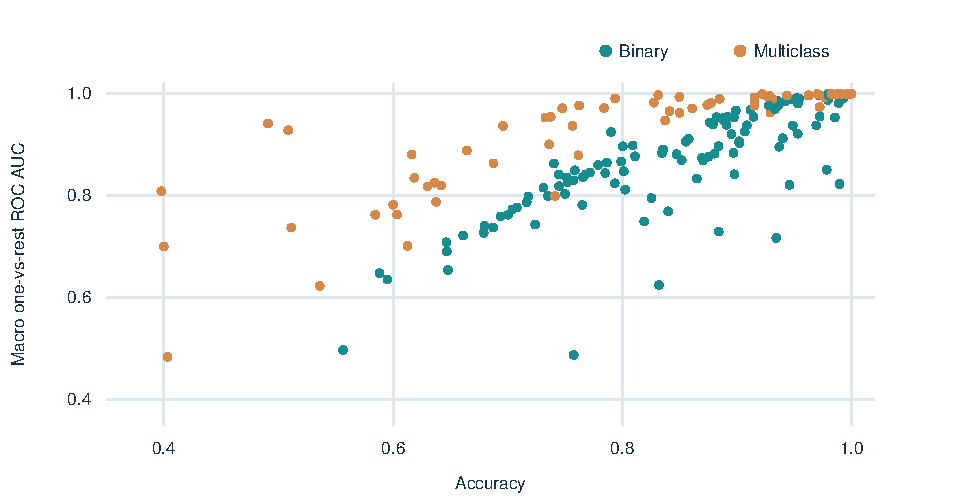
\includegraphics[width=\columnwidth]{figures/talent_accuracy_auc.pdf}
\caption{Accuracy versus macro one-vs-rest AUC for the 188 completed TALENT tasks, reproduced from the team benchmarking report~\cite{talentreport}, p. 3.}
\label{fig:talentauc}
\end{figure}
Binary tasks have higher mean accuracy but multiclass tasks have higher mean macro AUC. This is descriptive, not a controlled effect of task type. For example, \texttt{UJI\_Pen\_Characters} has 49.08\% accuracy despite AUC 0.9416 and log loss 1.8298; \texttt{drug\_consumption} attains AUC 0.4843. The low-accuracy tasks are retained in the aggregates. Without class frequencies or predictions, the causes cannot be established.

\subsection{Runtime Analysis}
The reported mean runtime is 79.41 s, compared with a median of 12.57 s; successful evaluations total 14,928.96 s (4.15 h). The right tail is substantial, with the slowest task taking 1,260.34 s. Figure~\ref{fig:talentruntime} relates runtime to training size. These timings exclude loading, downloads, metric calculation, export and unsuccessful attempts, and were collected without explicit CUDA synchronisation; they are application-level measurements rather than kernel timings or total notebook wall-clock time.
\begin{figure}[t]
\centering
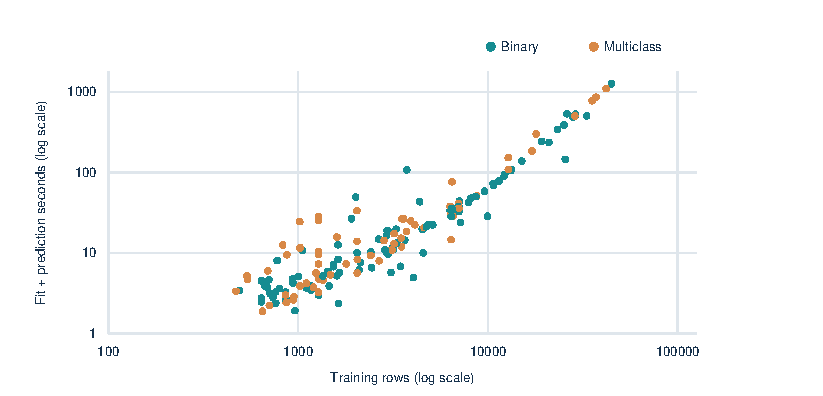
\includegraphics[width=\columnwidth]{figures/talent_runtime.pdf}
\caption{Fit-plus-probability-prediction runtime versus training rows (log scales), reproduced from the team benchmarking report~\cite{talentreport}, p. 4.}
\label{fig:talentruntime}
\end{figure}
\begin{table}[t]
\caption{Five Slowest Completed TALENT v1 Tasks}
\centering\footnotesize
\begin{tabular}{@{}p{0.53\columnwidth}rr@{}}\toprule
Dataset & Train rows & Seconds\\\midrule
Cardiovascular-Disease-dataset &44,800&1260.34\\
internet\_firewall &41,940&1099.14\\
shuttle &37,120&856.77\\
BNG(cmc)&35,388&776.37\\
adult&26,048&533.51\\\bottomrule
\end{tabular}
\end{table}

\subsection{Relationship to the Specialist Experiment}
\begin{table}[t]
\caption{Two Distinct Experimental Protocols}
\label{tab:protocols}
\centering\footnotesize
\begin{tabular}{@{}p{0.25\columnwidth}p{0.32\columnwidth}p{0.33\columnwidth}@{}}\toprule
Property & TALENT benchmark & Specialist study\\\midrule
Model & Original v1 & Original v2 and experts\\
Tasks & 188 completed / 200 & 14 held out / 67\\
Task types & Binary and multiclass & Numerical binary\\
Rows & Full official train/test & 256 support / 128 query from training arrays\\
Estimators & 32 & 1 per model\\
Hardware & Tesla T4 & RTX 3050 Laptop\\
AMP & Off & On\\\bottomrule
\end{tabular}
\end{table}
The accuracy of 83.48\% in the broad v1 benchmark must not be compared as a treatment effect against 86.33\% for nearest top-three v2 routing. Model version, dataset inventory, partitions, context size, ensemble count and hardware differ. No matched v1/v2 speedup or specialist benchmark on all 200 tasks is available. The original TabICL paper~\cite{tabiclppr} considers a different comparative subset (171 datasets with at most ten classes, according to the supplied benchmarking report); our independent run does not reproduce its comparative baselines or significance tests.



\section{Qualitative Diagnostics}

The resampling experiment produced similarity plots for both mean and mean+std pooling.

These plots help determine whether representations remain consistent when different subsets of the same dataset are sampled.

\begin{figure}[t]
\centering
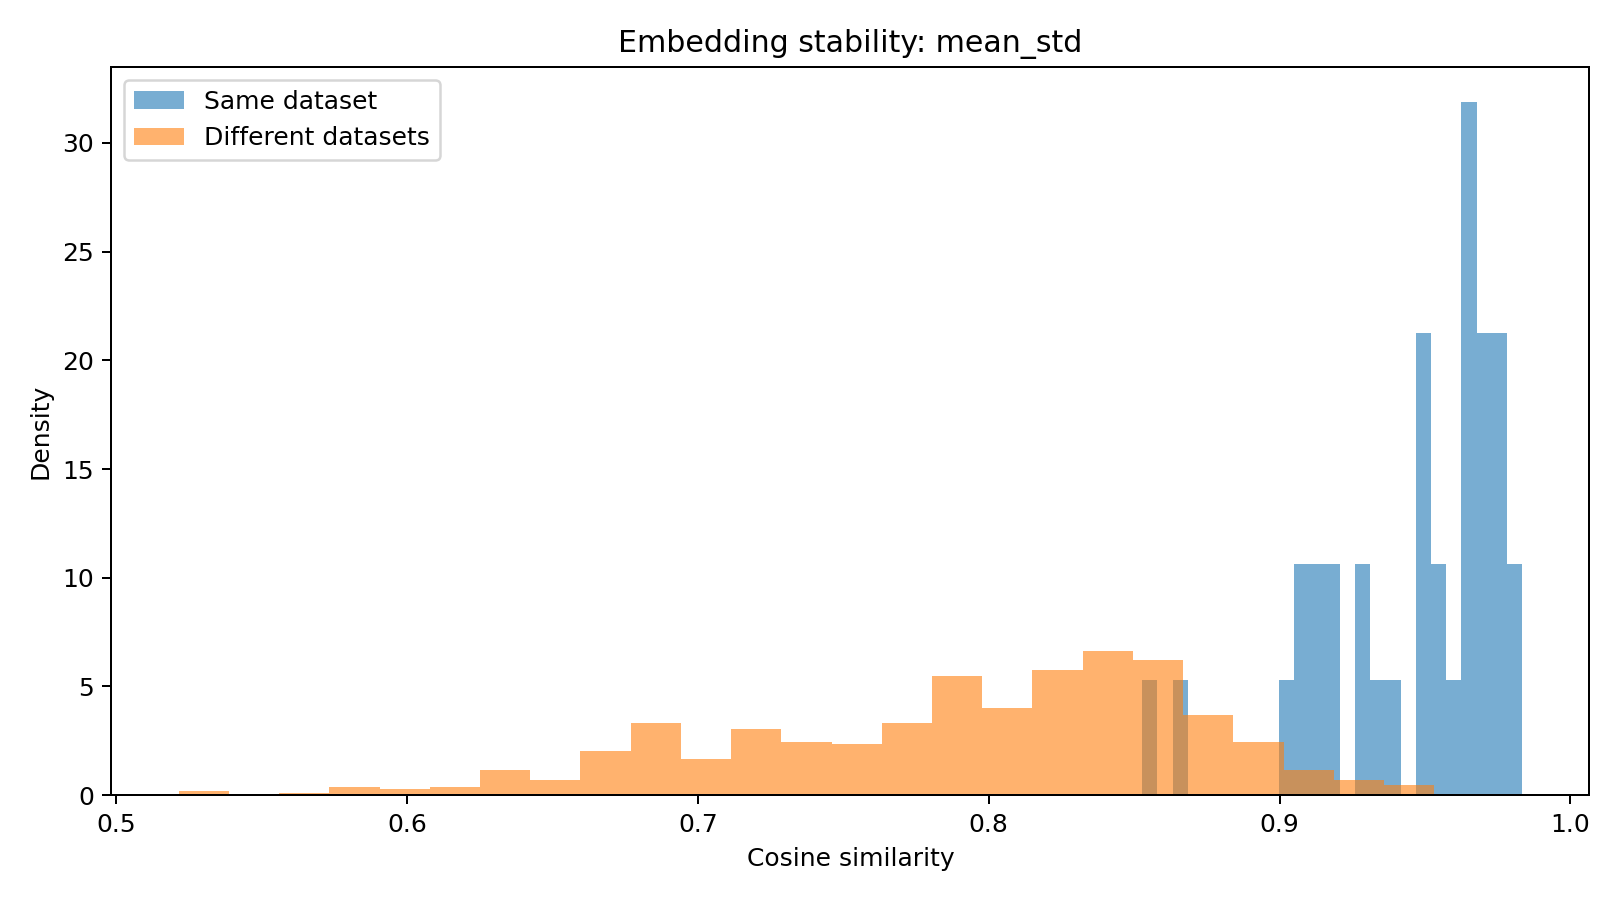
\includegraphics[width=\columnwidth]{figures/similarity_mean_std.png}
\caption{Cosine similarity diagnostic for 1024D mean+std pooled TabICL embeddings.}
\label{fig:similarity_meanstd}
\end{figure}

Although mean+std pooling provides high within-dataset similarity, it also increases similarity between different datasets.

Its within-versus-between similarity gap is 0.153, compared with 0.191 for mean pooling.

This motivates retaining mean pooling as the primary representation.

The robust-scaled statistical PCA projection provides another important observation.

\begin{figure}[t]
\centering
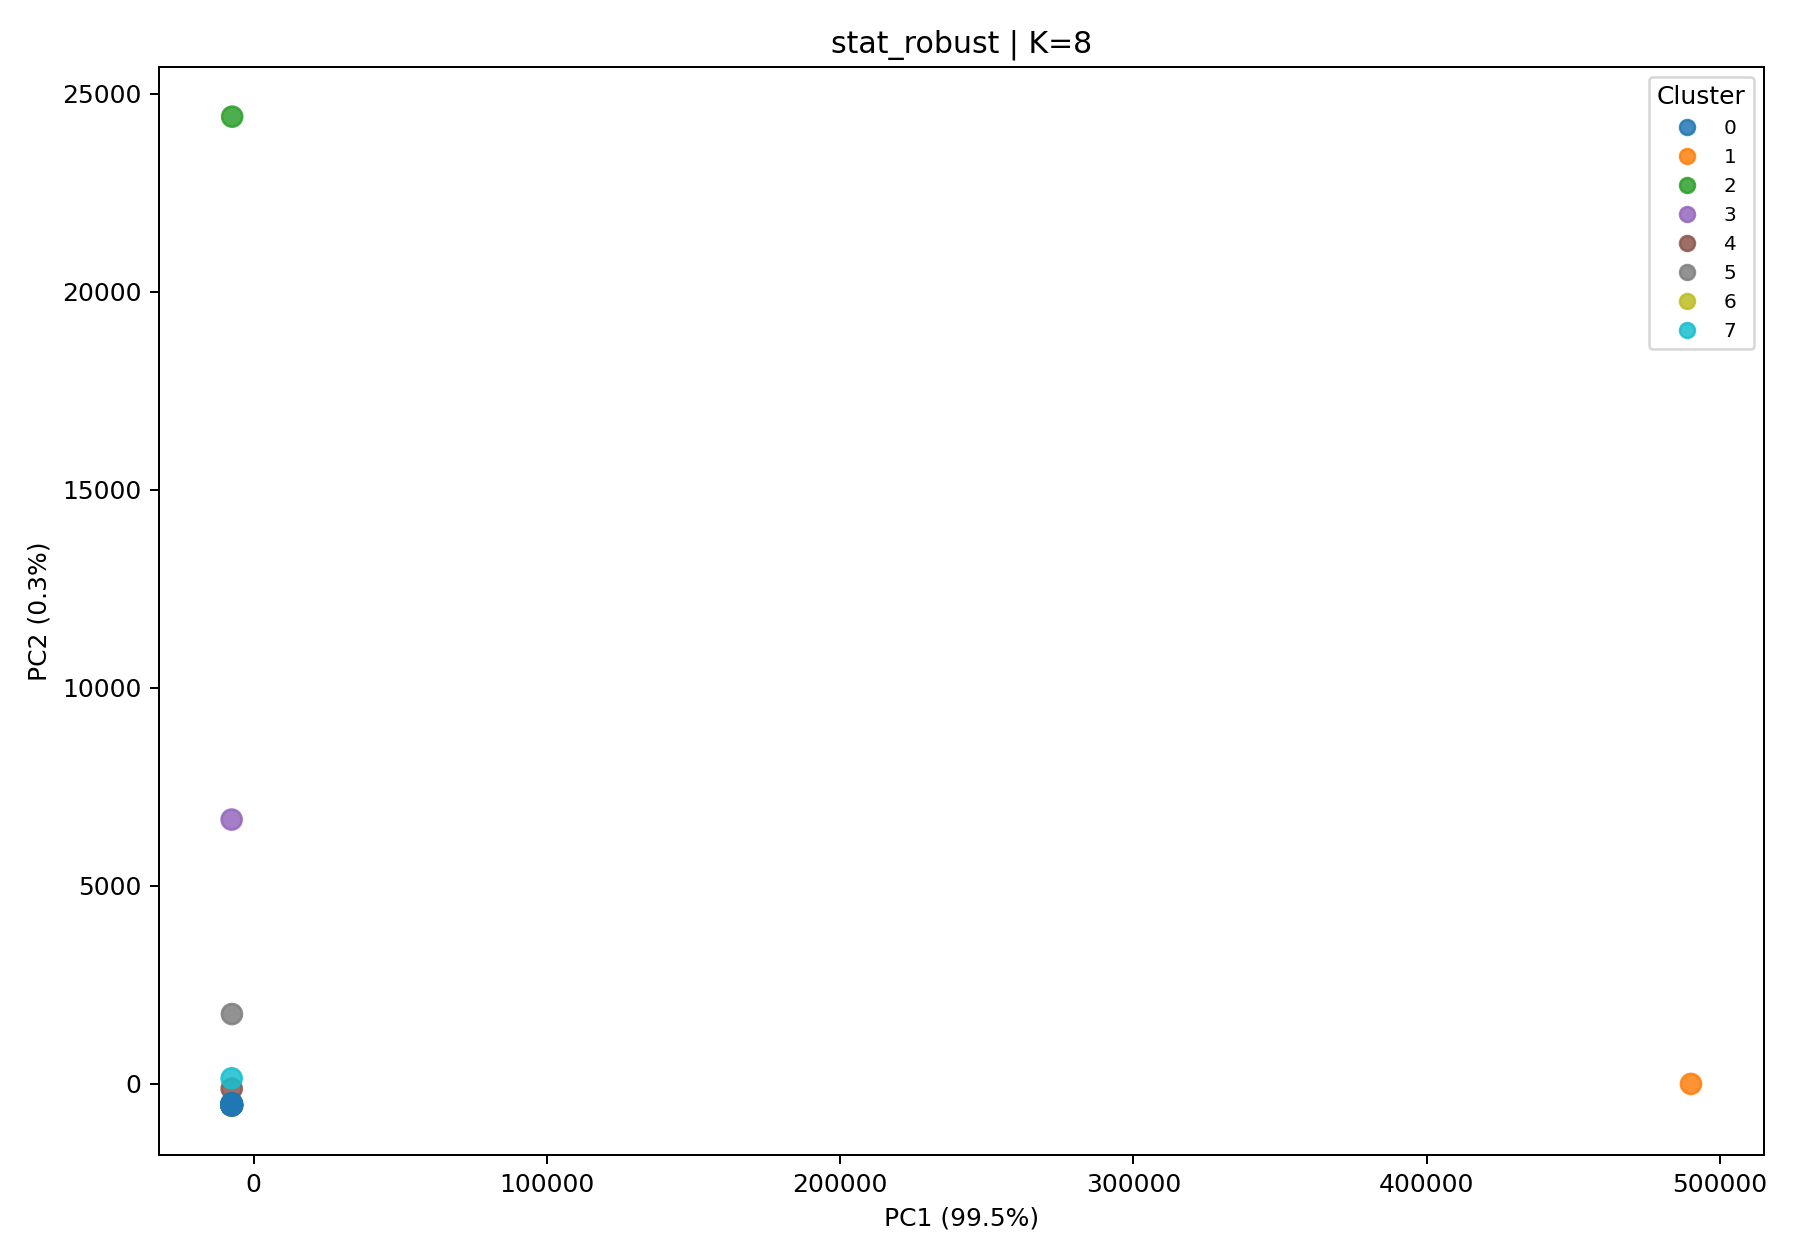
\includegraphics[width=\columnwidth]{figures/pca_stat_robust.png}
\caption{Exploratory PCA projection of robust-scaled statistical meta-features for K=8. The associated partition contains a 57-dataset cluster and six singleton clusters.}
\label{fig:pca_robust}
\end{figure}

Despite achieving a high silhouette score, robust-scaled statistical clustering creates highly imbalanced groups.

Such groups would be unsuitable for the intended multi-dataset expert training.

These observations demonstrate the importance of evaluating representation discrimination and cluster balance alongside conventional clustering metrics.

\section{Reproducibility and Implementation}
The consolidated team implementation~\cite{project} is available at \url{https://github.com/Mahidhar21/Dataset-Specialised-TabICL}. All three team contributions were integrated through pull request 1, which the project team reports has been merged into the main branch. The integration commit is \texttt{9c00a38}. The repository contains the following components:
\begin{itemize}
\item \path{dataset_representation_and_clustering/}: statistical meta-features, TabICL embeddings, stability analysis, clustering, family-aware splits and exploratory outputs.
\item \path{expert_training_and_routing/}: shared utilities, frozen routing manifest, embedding extraction, router fitting, episodic expert training, prediction and routing ablations.
\item \path{talent_benchmarking/}: independent TabICL v1 Colab notebook and execution instructions.
\item \path{results/}: expert configurations and training histories, per-dataset evaluations, routing selections, aggregate metrics, TALENT workbook and benchmarking report.
\item \path{report/}: consolidated LaTeX manuscript and figures.
\end{itemize}
The root README documents reproduction commands. The environment versions are recorded in \path{requirements.txt}, and the upstream TabICL revision in \path{tabicl_upstream_commit.txt}. The specialist implementation uses TabICL 2.2.0 and internal fine-tuning APIs; the source is available at \url{https://github.com/soda-inria/tabicl}. The independent TALENT notebook pins commit \path{7ccaddaa45f9d586d90df37126d39a0cb2a964e7} and checkpoint \texttt{tabicl-classifier-v1-20250208.ckpt}. Its separate environment must be preserved.

\subsection{Reproduction and Integration Verification}
Run the specialist pipeline from the repository root using the appropriate Python/CUDA environment and the original numerical dataset arrays. Set \texttt{DATA} to the dataset directory. The README covers embedding extraction, router fitting, training of experts 0--3 and evaluation of all routing controls. For example, the module entry points are:
\begin{lstlisting}[basicstyle=\ttfamily\scriptsize,breaklines=true,frame=single]
python -m expert_training_and_routing.extract_embeddings --data-dir "$DATA" --device cpu
python -m expert_training_and_routing.build_router
for i in 0 1 2 3; do
  python -m expert_training_and_routing.train_experts --data-dir "$DATA" --expert "$i" --epochs 3 --steps-per-epoch 30 --rows 64 --features 32 || break
done
python -m expert_training_and_routing.evaluate --data-dir "$DATA" --max-datasets 0 --top-k 3
\end{lstlisting}
After restructuring, Python and notebook syntax checks passed, and all five downstream module command-line interfaces loaded successfully. A two-dataset inference smoke test reused the frozen router and expert checkpoints, with zero failures. The observed per-dataset accuracies and selected expert indices matched the original results for the two tested tasks, as shown in Table~\ref{tab:smoke}. This check does not establish equivalence on all datasets or constitute a full retraining or TALENT rerun.
\begin{table}[t]
\caption{Post-integration Inference Smoke Test (Accuracy, \%)}
\label{tab:smoke}
\centering\footnotesize
\begin{tabular}{lrrr}\toprule
Dataset & Pretrained & Top-1 & Top-3\\\midrule
Microwave 10.0 GHz & 89.84 & 88.28 & 90.62\\
Microwave 10.5 GHz & 92.97 & 92.19 & 92.19\\\bottomrule
\end{tabular}
\end{table}
The frozen baseline archive contains the downstream code, regenerated embeddings, router, expert checkpoints and evaluation artifacts; its SHA-256 checksum was verified. Large checkpoints, generated embeddings, fitted router objects and original dataset arrays are kept outside ordinary Git. The original benchmark arrays and upstream pretrained checkpoint must be obtained separately. The TALENT workbook and report are included, but the original 188 per-task JSON records are not available for independent verification. Full retraining, exploratory Stage 1--2 reruns and full TALENT benchmarking were not repeated after consolidation.

\section{Discussion and Limitations}
The representation experiments support a practical 512D mean-pooled, four-cluster prototype. The downstream experiments establish that independent multi-dataset fine-tuning and retrieval-based inference are feasible on a 6 GB GPU. They do not establish that dataset similarity predicts expert competence. In particular, one selected expert remains pretrained and the fixed ensemble is slightly stronger in accuracy than nearest routing.

The specialist study is restricted to numerical binary-classification tasks. Family grouping is heuristic, five meta-test datasets share a microwave-sensing family, and only one split and seed are reported. Validation groups are small, especially expert 3 (one dataset). Ordinary K-means does not guarantee balanced clusters, and K=4 and K=8 exploratory comparisons use different splits. The exploratory statistical imputation is not fully train-only. Moreover, the downstream data loader computes feature medians over the entire source training array before within-dataset support/query splitting; if missing values occur, this exposes query feature statistics. A stricter inductive evaluation must fit imputation on support rows only and regenerate embeddings and rerun all methods. The embedding hook additionally sees one unlabelled query row, excluded from pooling; a strictly support-only embedding should use a support-derived probe and verify independence from external queries. These limitations do not imply query labels were supplied to the predictor, but restrict the strength of generalisation claims.

The separate TALENT evaluation is subject to completion bias: tasks were scheduled by a size-based heuristic and the unfinished tasks are not a random subset. It reports one seed and configuration, without raw probabilities, labels, class proportions, memory measurements or full execution logs in the supplied materials. Therefore calibration, subgroup performance, independent AUC/log-loss recomputation and statistical significance are not established. Related datasets may also reduce independence. The workbook is an earlier snapshot than the 188-task benchmark report.

\subsection{Future Work}
Evaluate each expert on each held-out dataset to estimate oracle selection and routing regret for diagnosis only. Use independent meta-validation tasks for learning competence-aware routing or choosing hyperparameters. Compare against a single globally fine-tuned TabICL and the all-expert ensemble; repeat family-aware splits and report family-level uncertainty. Reevaluate statistical and alternative learned embeddings under identical data splits, expert training budgets, and prediction protocols. Use the official dataset test partitions and support-only preprocessing when available. Complete the pending TALENT runs and compare v1, v2 and specialists on matched tasks and support budgets before drawing comparative accuracy or runtime conclusions.

\section{Conclusion}
We implemented all four stages of a dataset-specialised TabICL architecture: representation extraction, clustering, independent expert training, and retrieval-based prediction. On 14 held-out datasets, nearest top-three aggregation obtains 86.33\% accuracy compared with 86.16\% for pretrained TabICL. Fixed top-three reaches 86.38\%, and pretrained TabICL remains strongest on the other reported metrics. The system is operational and competitive, but a reliable benefit from dataset-aware routing remains unproven. The independent TALENT benchmark additionally documents 83.48\% mean accuracy and 0.8936 macro AUC over 188 completed tasks with the v1 checkpoint and a different protocol. It supplies broader descriptive context rather than evidence of specialist superiority. The specialist baseline is preserved for reproducible future investigation.

\begin{thebibliography}{9}

\bibitem{tabicl}
TabICL project, ``TabICL: A tabular foundation model for in-context learning,'' software repository. [Online]. Available: \url{https://github.com/soda-inria/tabicl}

\bibitem{project}
A. Sri Nikesh, G. Mahidhar, and K. Deepak Reddy,
``Dataset-Specialised TabICL,''
MA 305 Data Science Project, Team 7, 2026.
[Online]. Available:
\url{https://github.com/Mahidhar21/Dataset-Specialised-TabICL}

\bibitem{deepsets}
M. Zaheer et al.,
``Deep Sets,''
in \emph{Advances in Neural Information Processing Systems},
2017.

\bibitem{kmeans}
J. MacQueen,
``Some methods for classification and analysis of multivariate observations,''
in \emph{Proceedings of the Fifth Berkeley Symposium on Mathematical Statistics and Probability},
1967, pp. 281--297.

\bibitem{silhouette}
P. J. Rousseeuw,
``Silhouettes: A graphical aid to the interpretation and validation of cluster analysis,''
\emph{Journal of Computational and Applied Mathematics},
vol. 20, pp. 53--65, 1987.

\bibitem{ari}
L. Hubert and P. Arabie,
``Comparing partitions,''
\emph{Journal of Classification},
vol. 2, pp. 193--218, 1985.

\bibitem{tabiclppr}
J. Qu, D. Holzm\"uller, G. Varoquaux, and M. Le Morvan, ``TabICL: A tabular foundation model for in-context learning on large data,'' in \emph{Proc. ICML}, PMLR 267, 2025.

\bibitem{talentreport}
Project Team, ``TabICL on the TALENT Benchmark: An empirical analysis of 188 completed classification tasks,'' internal experimental report, Nov. 18, 2026.

\bibitem{talentworkbook}
Project Team, \texttt{TALENT\_200.xlsx}, saved benchmark metrics, 187 scored task snapshot, Nov. 2026.

\end{thebibliography}

\end{document}